When working with unit operations that involve matrix operations dealing with vectors of different dimensions, the order in which we apply the chain rule matters \cite{Giering_Kaminski_1998}.
When computing a gradient using AD, we can encounter vector-Jacobian products (VJPs) or Jacobian-vector products (JVP).
As their name indicates, the difference between them is that the quantity we are interested in is described by the product of a Jacobian times a vector on the left side (VJP) or the right (JVP).
Furthermore, both forward and reverse AD can be thought of as a way of computing derivatives associated with JVPs (see Equation \eqref{eq:directional-derivative}) and VJPs, respectively. 
In other words, given a function $g: \R^{d_1} \mapsto \R^{d_2}$ that is evaluated during the forward mode of given program, AD will carry terms of the form $Dh (x) \cdot \dot x$ (JVP) in forward mode and $\bar y^T \cdot Dh (x)$ (VJP) in reverse mode \cite{Griewank:2008kh}.

Let us consider for example the case of a nested loss function $L : \mathbb R^p \mapsto \mathbb R$ taking a total of $p$ arguments as inputs that can be decomposed as $L(\theta) = \ell \circ g_{k} \circ \ldots \circ g_2 \circ g_1(\theta)$, with $\ell : \mathbb R^{d_k} \mapsto \mathbb R$ the final evaluation of the loss function after we apply in order a sequence of intermediate functions $g_i : \mathbb R^{d_{i-1}} \mapsto \mathbb R^{d_i}$, where we define $d_0 = p$ for simplicity. 
The final gradient is computed as the chain product of vectors and Jacobians as
\begin{equation}
 \nabla_\theta L = \nabla \ell \cdot Dg_{k} \cdot Dg_{k-1} \cdot \ldots \cdot Dg_2 \cdot Dg_1, 
\end{equation}
% \todo[inline]{Eqn (25) is misleading insofar as it gives the (wrong) impression that grad(L) can be computed in forward mode. But that is not the case. All that can be computed is grad(L)*v(0). The grads should be changed into "D", or you should make the product of grad(L)*v(o) explicit.
% You'll need the transpose of that eqn to get the gradient.}
with $Dg_i$ the Jacobian of each nested function evaluated at the intermediate values $g_{i-1} \circ g_{i-2} \circ \ldots \circ g_i (\theta)$.
Notice that in the last equation $\nabla \ell \in \mathbb R^{d_k}$ is a vector.
% \todo{See above comment: All that eqn (25) can do is solve grad(L)*v(0), ie the directional derivative.}
In order to compute $\nabla_\theta L$, we can solve the multiplication starting from the right side, which will correspond to multiplying the Jacobians forward from $Dg_1$ to $Dg_k$, or from the left side, moving backwards. 
The important aspect of the backwards case is that we will always be computing VJPs, 
% \todo{No, $\nabla \ell$ is not a vector, it's a gradient.}
since $\nabla \ell$ is a vector.
Since VJPs are easier to evaluate than full Jacobians, the reverse mode will in general be faster when $1 \ll p$. This example is illustrated in Figure \ref{fig:vjp-jvp}. 
% \todo[inline]{JVPs are also easier to evaluate than Jacobians. The point is that JVP maps from dim(p) to dim(1), whereas VJP maps from dim(1) to dim(p).}
For general rectangular matrices $A\in \mathbb R^{d_1 \times d_2}$ and $B \in \mathbb R^{d_2 \times d_3}$, the cost of the matrix multiplication $AB$ is $\mathcal O (d_1 d_2 d_3)$.

It is worth noting that while more efficient methods for matrix-matrix multiplication based on Strassen’s recursive algorithm and its variants exist, these are not extensively used in most scientific applications \cite{Silva_Gustafson_Wong_2018, Huang_Smith_Henry_Geijn_2016}.
This implies that forward AD requires a total of
\begin{equation}
 d_2 d_1 p + d_3 d_2 p + \ldots + d_k d_{k-1} p + d_k p = \mathcal O (kp)
\end{equation}
operations, while backwards mode AD requires
\begin{equation}
 d_k d_{k-1} + d_{k-1} d_{k-2} + \ldots + d_2 d_1 + d_1 p = \mathcal O (k+p)
\end{equation}
operations. 

In the general case of a function $L : \R^p \mapsto \R^q$ with multiple outputs and a total of $k$ intermediate functions, the cost of forward AD is $\mathcal O (pk + q)$ and the cost of reverse is $\mathcal O (p + kq)$.
When the function to differentiate has a larger input space than output ($q \ll p$), AD in reverse mode is more efficient as it propagates the chain rule by computing VJPs.
For this reason, reverse-mode AD is preferred in both modern machine learning and inverse methods.
However, notice that reverse mode AD requires saving intermediate variables through the forward run in order to run backwards afterwards \cite{Bennett_1973}, leading to performance overhead that makes forward AD more efficient when $p \lesssim q$ \cite{Griewank_1989, Margossian_2018, Baydin_Pearlmutter_Radul_Siskind_2015}. 

\begin{figure}[t]
    \centering
    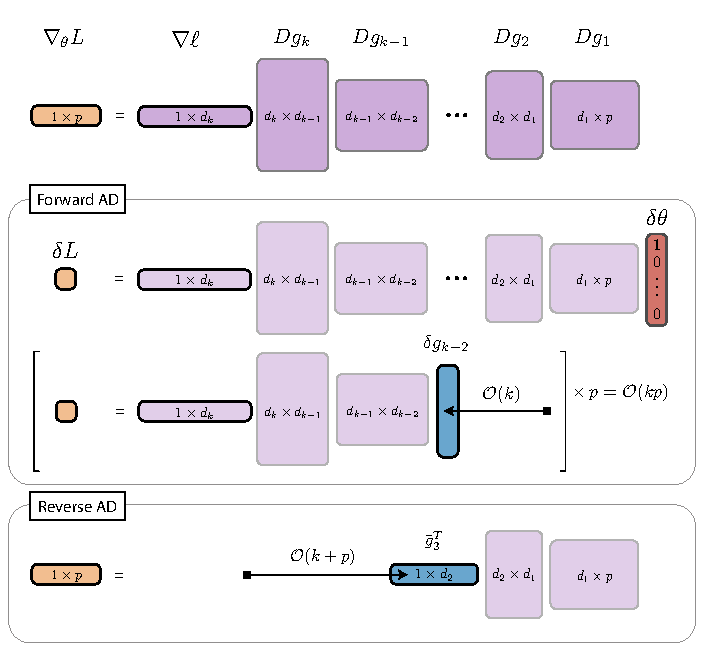
\includegraphics[width=0.95\textwidth]{figures/VJP-AD.pdf}
    \caption{Comparison between forward and reverse mode AD. Changing the order of Jacobian multiplications changes the total number of floating-point operations, which leads to different computational complexities between forward and reverse mode. When the multiplication is carried from the right side of the mathematical expression for $\nabla_\theta L$, each matrix simplification involves a matrix with size $p$, giving a total complexity of $\mathcal O (kp)$. This is the opposite of what happens when we carry the VJP from the left side of the expression, where the matrix of size $d_1 \times p$ has no effect in the intermediate calculations, making all the intermediate calculations $\mathcal O (1)$ with respect to $p$ and a total complexity of $\mathcal O (k + p)$. }
    % However, backwards mode requires storing in memory information about the forward execution of the program, while forward mode can update the gradient on running time.}
    \label{fig:vjp-jvp}
\end{figure}

In practice, many AD systems are reduced to the computation of only directional derivatives (JVPs) or gradients (VJPs) \cite{Griewank:2008kh}.
Full Jacobians $J \in \R^{n \times p}$ (e.g., the sensitivity $s = \frac{\partial u}{\partial \theta} \in \R^{n \times p}$) can be fully reconstructed by the independent computation of the $p$ columns of $J$ via the JVPs $J e_i$, with $e_i \in \R^p$ the canonical vectors; or by the calculation of the $m$ rows of $J$ via the VJPs $e_j^T J$, with $e_j \in \R^n$.
Sparse Jacobians are commonplace in large-scale nonlinear systems and discretized PDEs. % Reference here!
When the sparsity pattern is known, they can be efficiently obtained with \textit{colored AD} to chunk multiple JVPs or VJPs, based on the colored Jacobian~\cite{gebremedhin2005color}.
More concretely, consider the example of a Jacobian, ${J}_{\text{sparse}}$, with known sparsity pattern given by
\begin{equation}
    {J}_{\text{sparse}} = \begin{bmatrix}
        \bullet &         &         &         &         \\
                & \bullet & \bullet &         &         \\
                &         &         & \bullet &         \\
        \bullet & \bullet &         &         & \bullet \\
                &         &         &         & \bullet
    \end{bmatrix},
\end{equation}
where $\bullet$ denotes the non-zero elements of the Jacobian. 
% AD tools compute Jacobians column-wise or row-wise by composing multiple JVPs or VJPs respectively. 
% This is done to avoid perturbation confusion~\cite{manzyuk2019perturbation}. 
We can color the above matrix as follows: % This requires more explanation
\begin{equation}
    {J}^{(\text{col})}_{\text{sparse}} = \begin{bmatrix}
        \color{myred}{\blacktriangleright} &                            &                                  &                                  &                              \\
                                         & \color{myblue}{\blacksquare} & \color{myred}{\blacktriangleright} &                                  &                              \\
                                         &                            &                                  & \color{myred}{\blacktriangleright} &                              \\
        \color{myred}{\blacktriangleright} & \color{myblue}{\blacksquare} &                                  &                                  & \color{myviolet}{\blacklozenge} \\
                                         &                            &                                  &                                  & \color{myviolet}{\blacklozenge}
    \end{bmatrix} \qquad {J}^{(\text{row})}_{\text{sparse}} = \begin{bmatrix}
        \color{myblue}{\blacksquare}   &                              &                            &                            &                              \\
                                     & \color{myblue}{\blacksquare}   & \color{myblue}{\blacksquare} &                            &                              \\
                                     &                              &                            & \color{myblue}{\blacksquare} &                              \\
        \color{myviolet}{\blacklozenge} & \color{myviolet}{\blacklozenge} &                            &                            & \color{myviolet}{\blacklozenge} \\
                                     &                              &                            &                            & \color{myblue}{\blacksquare}
    \end{bmatrix}.
\end{equation}
To compute $J^{(\text{col})}_{\text{sparse}}$, we just need to perform three JVPs, 
\begin{equation}
    J^{(\text{col})}_{\text{sparse}} 
    \begin{bmatrix}
    1 \\ 0 \\ 1 \\ 1 \\ 0    
    \end{bmatrix}
    = 
    \begin{bmatrix}
    \color{myred}{\blacktriangleright} \\ \color{myred}{\blacktriangleright} \\ \color{myred}{\blacktriangleright} \\ \color{myred}{\blacktriangleright} \\ \\   
    \end{bmatrix}, \qquad
    J^{(\text{col})}_{\text{sparse}} 
    \begin{bmatrix}
    0 \\ 1 \\ 0 \\ 0 \\ 0    
    \end{bmatrix}
    = 
    \begin{bmatrix}
    \\ \color{myblue}{\blacksquare} \\ \\ \color{myblue}{\blacksquare} \\ \\ 
    \end{bmatrix}, \qquad
    J^{(\text{col})}_{\text{sparse}} 
    \begin{bmatrix}
    0 \\ 0 \\ 0 \\ 0 \\ 1    
    \end{bmatrix}
    = 
    \begin{bmatrix}
    \\ \\ \\ \color{myviolet}{\blacklozenge} \\ \color{myviolet}{\blacklozenge} \\ 
    \end{bmatrix},
\end{equation}
compared to five JVPs for a $5 \times 5$ dense Jacobian.
Similarly, since reverse mode materializes the Jacobian one row at a time, we need two VJPs (once each for $\color{myblue}{\blacksquare}$, and $\color{myviolet}{\blacklozenge}$) compared to five VJPs for the dense counterpart. 